\chapter{Installations and datasets}

\begin{figure}[h]
\centering
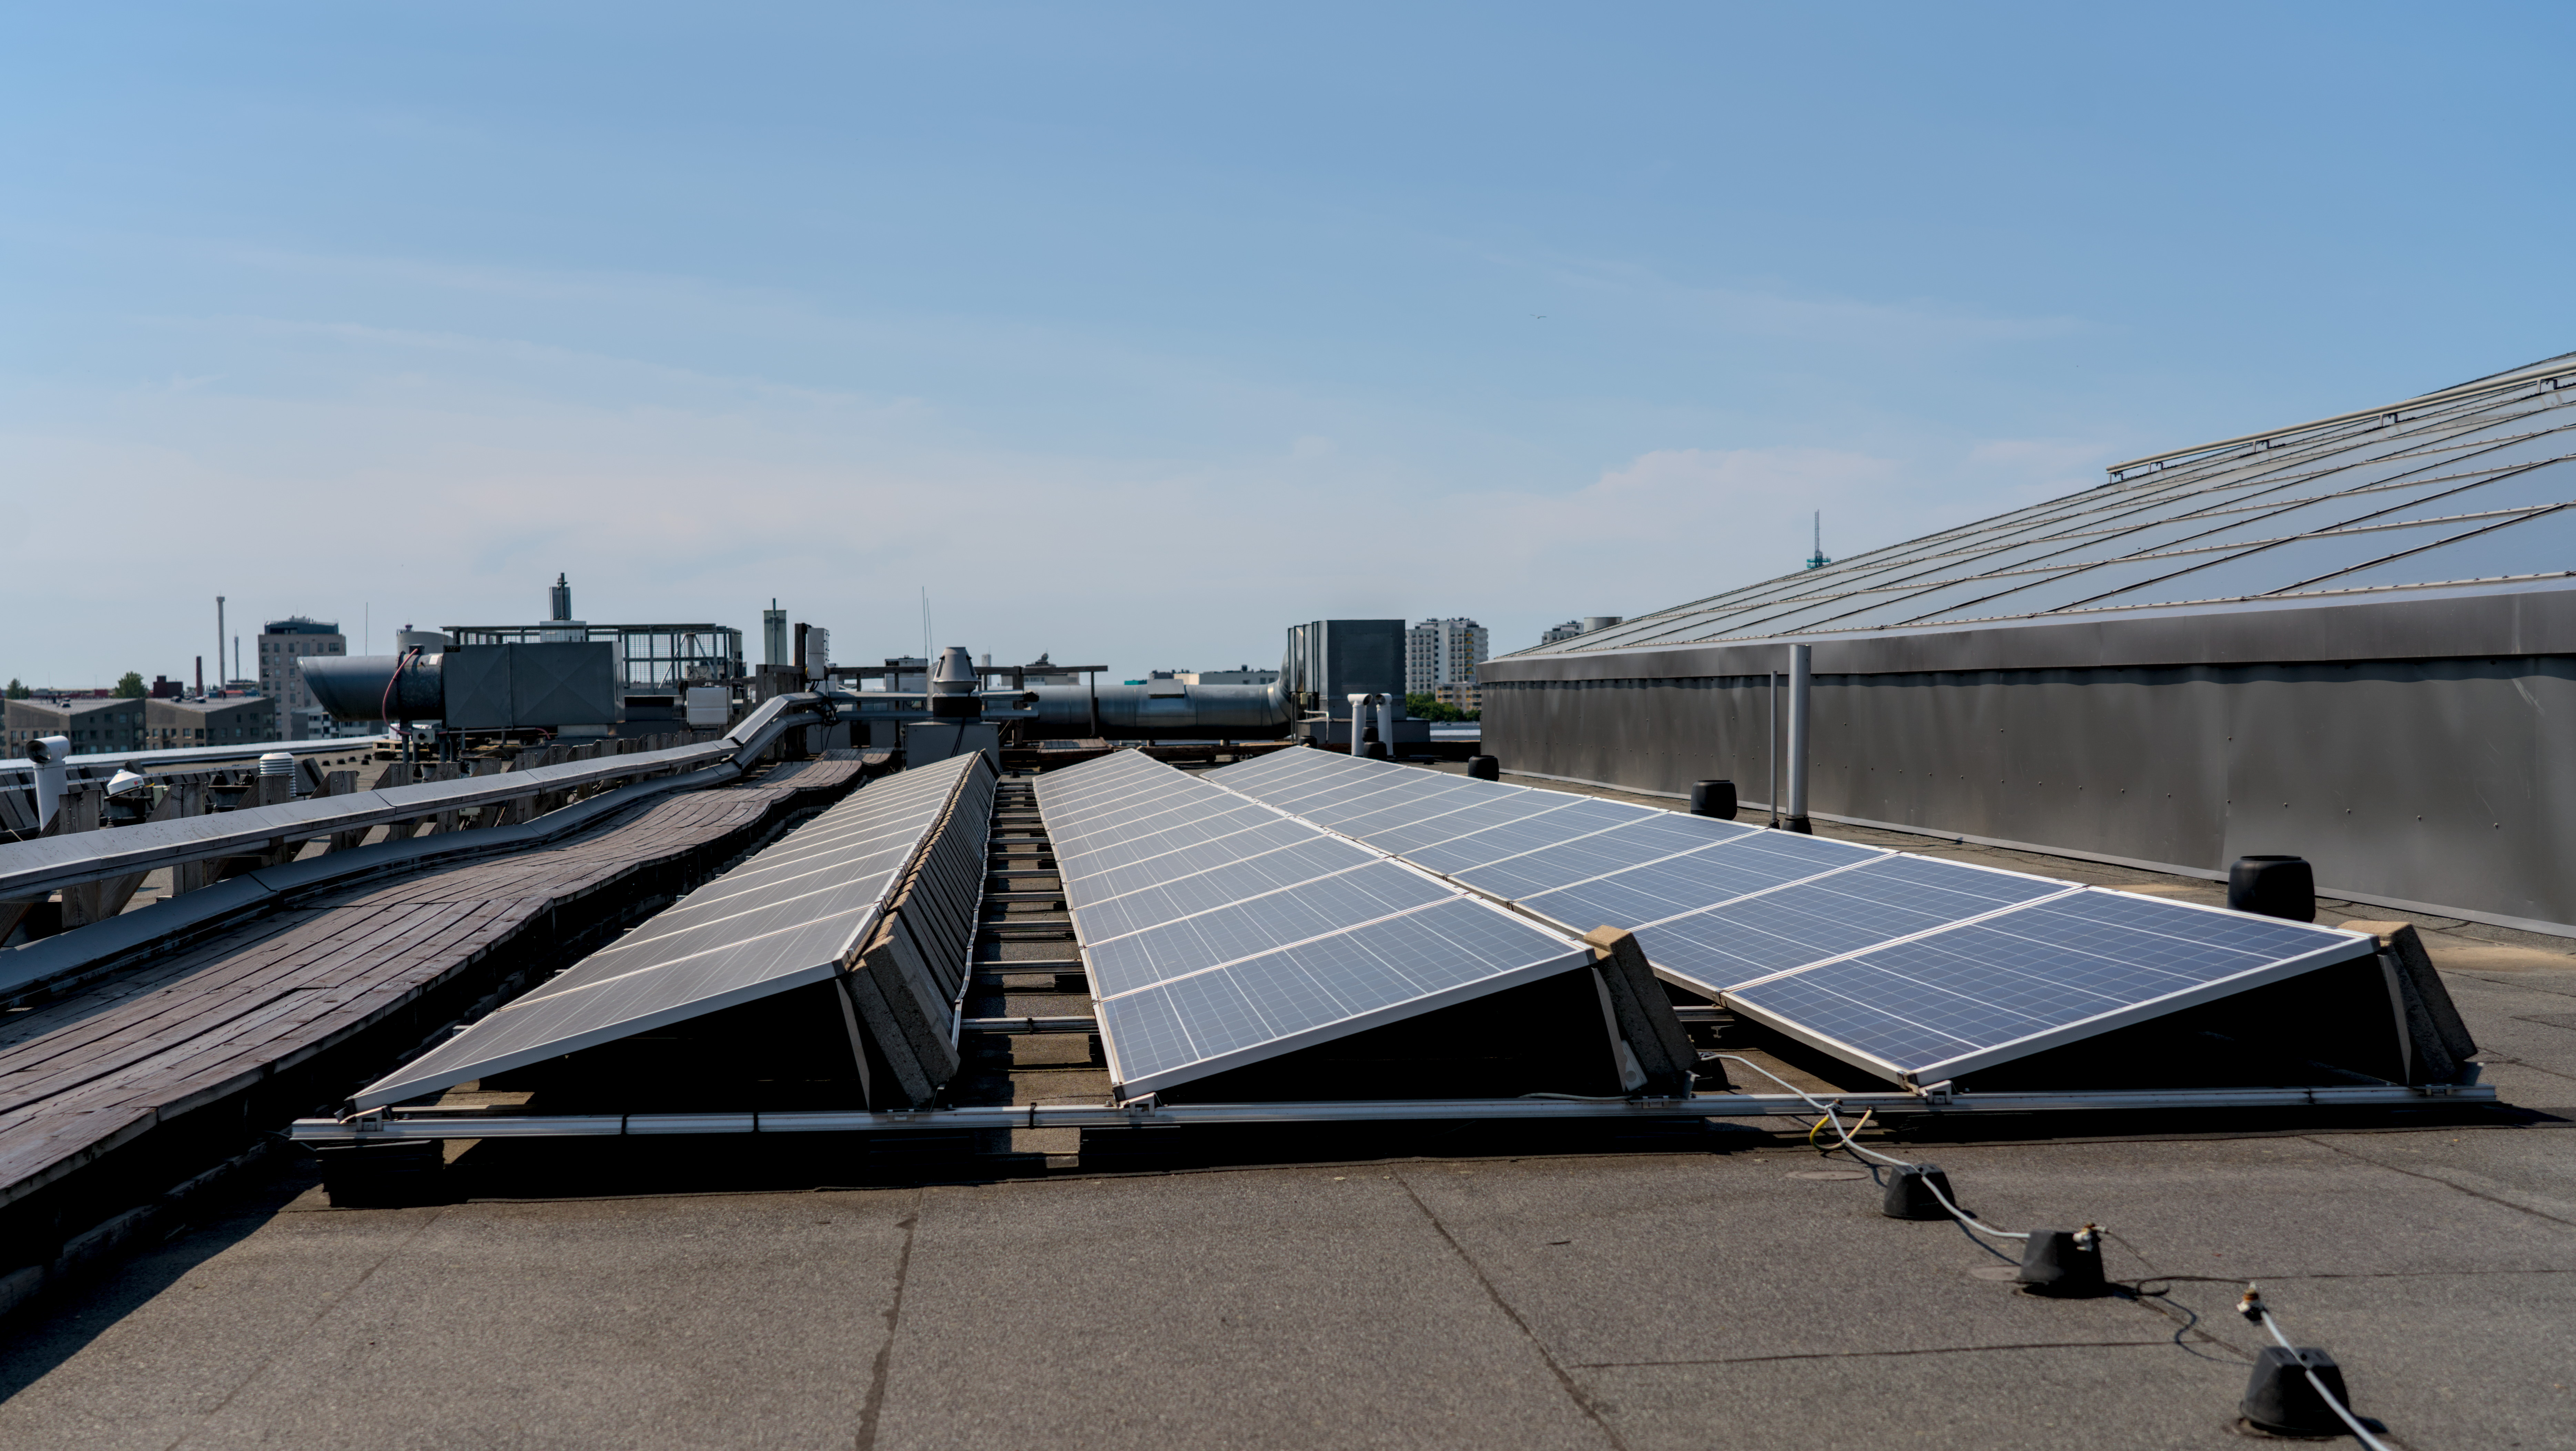
\includegraphics[width=0.8\linewidth]{pics/fmikumpula}
\figcaption{FMI Kumpula solar power installation string.}
\label{fig_fmikumpula_panels}
\end{figure}


\noindent The two datasets used in theis thesis were provided by FMI. They contain power generation measurements from installations in Kuopio and Helsinki, with the physical parameters listed in table \ref{table_fmi_helsinki_kuopio_parameters}. Due to the high elevation of the installations, shading is unlikely to be a major factor in either of the datasets. The same data was previously used in Herman Böök's \textit{Photovoltaic output modeling}\cite{hbook1} and thus installation parameters and datasets have previously been verified.

Data in the two datasets follows a similar structure as shown in table \ref{table_fmi_kumpula_csv}. This snapshot from the Helsinki dataset shows that the temporal resolution is one measurement per minute and that there are multiple power values for each minute. The fields \textit{String 1} and \textit{String 2} represent power from two identical sets or strings of solar PV panels installed at the same location and their sum should be near equal to inverter input. One of these strings is shown in figure \ref{fig_fmikumpula_panels}. Datasets from other sources may differ from the FMI datasets in several ways. Power measurements may be taken at different intervals, once per 1, 5, 15, or 60 minutes and they are unlikely to contain more than one power value. Due to these reasons, the algorithms in this thesis are designed to operate on datasets with one measurement per minute and they use only the inverter output value as that is the most likely power value included in solar PV datasets.


%Other datasets may differ from FMI datasets. The most likely differences are temporal resolution and the amount of included power measurement points. As the inverter output is the most important value for end users, this will be the only power value used by the algorithms. %The temporal resolution of one measurement per minute in FMI datasets is likely to be higher than that of most PV datasets, but  

% As these installations are used for research purposes, the temporal resolution and amount of power measurements are likely to be different from other solar PV datasets. Due to this, the algorithms in this thesis use the inverter output power value as it is the most likely power value to be included in datasets. The forementioned 


% As the inverter output describes the amount of power available to the user of a PV system, this will be used by the algorithms in the thesis. 


%ir data quality is likely to be higher than that of most regular solar PV installations. The multiple power measurements, installation metadata quality and 



%Having multiple power values has uses for data verification and analysis but the most relevant power value for the users of PV systems is the inverter output value and thus it is the value most likely to be included in datasets. 


%nother possible difference between FMI datasets and other datasets is the temporal resolution


%as the users of PV systems are interested in available power and thus inverter output values are the 


% only the inverter output value is likely to be included in solar PV datasets and thus it is the power value used in this thesis. Another possible difference between FMI datasets and other datasets is the temporal resolution as one measurement per minute 


% may be recorded anywhere from once per second to once per hour. Temporal resolution differences 
%The resolution of measurement per minute in FMI datasets should be accurate enough to allow for precise geolocation and panel installation estimation.




%have uses for analysis and data verification but are unlikely to be included in other datasets and thus algorithms in this thesis utilize only timestamps and inverter output values. Another likely difference between the datasets in this thesis and most real world datasets is the temporal resolution as power generation measurements may be recorded anywhere from once per second to once per hour. The resolution of measurement per minute in FMI datasets should be accurate enough to allow for precise geolocation and panel installation estimation.


\begin{table}[h]

\centering

\begin{tabular}{r|cccc} \hline\hline

Timestamp[UTC] & Inverter out & Inverter in & String 1 & String 2\\ \hline
$2015-08-26$ $03:34$ & $NaN$ & $NaN$ & $0.5$ & $NaN$\\
$2015-08-26$ $03:36$ & $11.1$ & $7.5$ & $2.6$ & $4.9$\\
$2015-08-26$ $03:37$ & $25.4$ & $26.1$ & $9.8$ & $16.3$\\
$2015-08-26$ $03:38$ & $30.7$& $NaN$ & $NaN$ & $0.4$\\
$2015-08-26$ $03:39$ & $46.4$& $44.8$ & $20$ & $24.8$\\
$2015-08-26$ $03:40$ & $3.3$ & $NaN$ & $NaN$ & $0.4$\\
$2015-08-26$ $03:41$ & $29.3$ &  $18$ & $9.1$ & $8.9$\\
$2015-08-26$ $03:42$ & $33.1$& $27.4$ & $10.6$ & $16.9$\\

\vdots & \vdots & \vdots & \vdots & \vdots\\
$2015-08-26$ $12:42$ & $12374.8$ & $14619.1$ & $7152$ & $7467.1$\\
$2015-08-26$ $12:43$ & $15442.2$ & $15482.1 $& $7708.9$ & $7773.2$\\
$2015-08-26$ $12:44$ & $14085.8$ & $12898.7$ & $6387$ & $6511.8$ \\
\vdots & \vdots & \vdots & \vdots & \vdots\\

\hline\hline
\end{tabular}

\tabcaption{A section from FMI's Kumpula solar site PV production data, only the timestamp and inverter output values are used by the algorithms in this thesis. All power measurements are in watts.}
\label{table_fmi_kumpula_csv}
\end{table}

%The same table shows that measurements for certain minutes are missing and that some values are recorded as NaN, Not-a-Number. Without proper preprocessing, mathematical operations such as sum, division and addition would be poorly defined and thus the dataset would be unusable. The required preprocessing is done by the removal of rows with NaN values and linear interpolation for filling out the resulting gaps. Filling gaps in the data is not necessary, but certain algorithms can be written more efficiently when no gaps are present.




%The table \ref{table_fmi_kumpula_csv} shows the general structure of solar PV energy output datasets with timestamps and power output values. The differences between FMI datasets and datasets from other sources are likely to be the timestamp formats, temporal resolution, power measurement units and the amount of different power measurement sources. Fields \textit{Inverter in}, \textit{String 1} and \textit{String 2} have uses for analysis and data verification but they or similar values to them are unlikely to be included in other datasets and thus this thesis utilize only timestamps and inverter output values.






%The algorithms in this thesis will work on any dataset with timestamps and power values, but the temporal resolution is likely to influence the accuracy of algorithms and interpolation has to be done in order to match the time resolution of measurements and the algorithms. The table also shows that the dataset is missing some values. In the case of the first and last daily minutes, this could be the result of the inverter or other instruments turning off when electricity generation is close to zero, but there could be other reasons as well. Due to the possibility of missing measurements and presence of NaN-values, the data has to be preprocessed. 


% similar data structures could be assumed to be the default in solar power generation datasets. The biggest difference between datasets could be assumed to be the temporal resolution, for example measurements for the power values could be taken every 15 minutes instead of every minute.



%Another point of interest are the multiple different power values included in the datafile. Columns String 1 and String 2 correspond to the output power from two identical sets of solar panels installed in the same installation site. Having two indentical installations at the same location has some value for data verification as both panel strings should provide almost identical outputs, but this is not the main focus of the thesis and thus these values are ignored. There are also two inverter values. The inverter input value is one step closer to the power generation of solar PV systems and thus algorithms that utilize this input value could be more accurate. However as the inverter output represents the amount of usable power generated by the PV system, the output is the most likely power value to be included in datasets and thus it will be used in this thesis.


%The table columns string 1 and string 2 correspond to the power outputs of two sets of panels. The output of these panels is used as the input of the inverter and thus the sum of string 1 and string 2 should closely match the inverter input value. The inverter is an electric device which converts the voltage of the solar panels so that the power generated by the solar panels can be fed into the electrical system of a home or some other facility.%As this output to an electric system is the best description of the power available to the user, an assumption can be made that the power value in other datasets refers to the inverter output unless otherwise indicated.



\begin{table}[H]
\centering
\begin{tabular}{r|cc} \hline\hline

 & Helsinki & Kuopio\\ \hline
 Latitude & $60.204^\circ$ & $62.892^\circ$ \\
 Longitude & $24.961^\circ$  &  $27.634^\circ$\\
 Nominal capacity &21 kW & 20.28 kW \\
 Panel tilt & $15^\circ$ & $15^\circ$ \\
 Panel angle & $135^\circ$ & $217^\circ$ \\
 Elevation & 17m & 10m\\
\hline\hline
\end{tabular}
\tabcaption{Parameters for the FMI's Kumpula(Helsinki) and Kuopio PV installations as listed in Böök 2020 \cite{hbook1}.}
\label{table_fmi_helsinki_kuopio_parameters}
\end{table}





\section{Visualizing the data}
The figure \ref{fig_oneyear_pointcloud} contains a 3D point cloud generated by plotting one year of data from FMI Helsinki dataset and it shows that there are patterns in the data. The clearest pattern is formed by the first and last non-zero power minutes and this pattern can be used for geolocation estimation. Similarly if one day slices from the dataset are taken as shown in \ref{fig_cloudfree_vs_cloudy}, the power generation plot shape can be later used for mathematical model fitting. However the difference between clear and cloudy or otherwise noisy days is significant and automating the process of cloud free day selection would be beneficial.



%free days is significant as seen in figure \ref{fig_cloudfree_vs_cloudy} and as cloudy or otherwise noisy days appear to be common in the data, automating the process of cloud free day selection is necessary.


%This shows that the timings of first and last non-zero power minutes appear to form a distinct pattern which is a result of changes in day length and this very same pattern can be used for geolocation estimation. If individual days from the dataset are plotted,



% Similarly the plot contains a noisy dome like-shape that can be used for analysis. In figure \ref{fig_cloudfree_vs_cloudy} we can see the the difference between different days in the dataset. This noise 



 %figure \ref{fig_cloudfree_vs_cloudy} 

\begin{figure}[h]
\centering
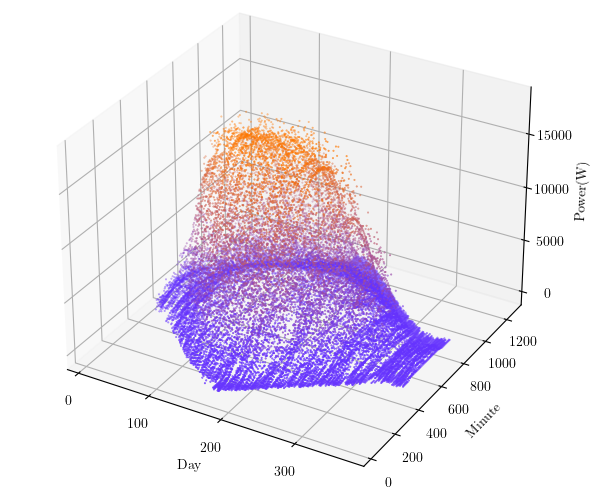
\includegraphics[width=0.8\linewidth]{pics/oneyear2}
\figcaption{One year of data from FMI Kumpula installation as a 3D point cloud.}
\label{fig_oneyear_pointcloud}
\end{figure}

\begin{figure}[h!]
\centering
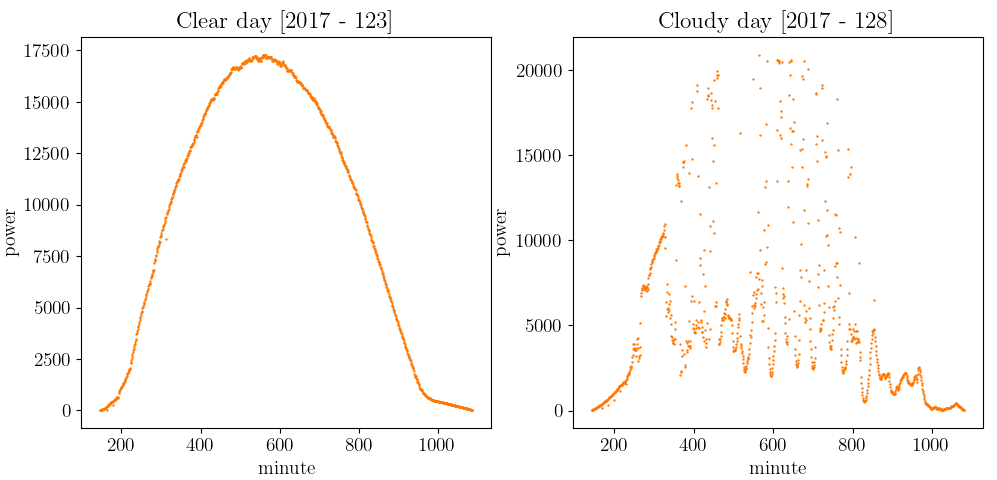
\includegraphics[width=1\linewidth]{pics/cloudfree_vs_cloudy}
\figcaption{Two days from FMI Kumpula dataset with different charasteristics.}
\label{fig_cloudfree_vs_cloudy}
\end{figure}

The cloud free day 2017-123 has some notable charasteristics in addition to the geolocation derived first and last minutes. The shape resembles a skewed normal distribution and the knee section near 950 minutes may signify a transition from direct solar irradiance to atmosphere scattered irradiance. Similarly intuition would suggest that the peak power minute is near the time when the angle between sun and the solar panel normal is at it's minimum. Measurable traits such as these could be used for parameter estimation, but the relationships between figure traits and system parameters can be complicated.



\newpage
\section{Data pre-processing}
The data pre-processing required by the algorithms in this thesis can be split into two gategories, classification and repairing. Classifying preprocessing is used to determine if a certain section of data is useful of analysis or not, the primary example here is the cloud free day detection algorithm which is discussed more throroughly in the next chapters. The second type of preprocessing, reparing preprocessing refers to the use of algorithms which fill in gaps or otherwise attempt to repair data which is unusable as is, but which could be used after repairing.


% Similarly algorithms can classify days as good and bad based on their measurement counts, legths or data gaps. 

The data preprocessing algorithms used in this thesis load the data from csv files and examine whether individual days in the dataset meet set qualifications. These are the minimum and maximum measurement count, whether first and last measurements are taken too close to minute 0 or 1440 and the the percentage of measurements included between the first and last measurement. Figure \ref{fig_accepted_days} shows which days met the set quality requirements.



\begin{figure}[h]
	
     \centering
     \begin{subfigure}[b]{0.48\textwidth}
         \centering
         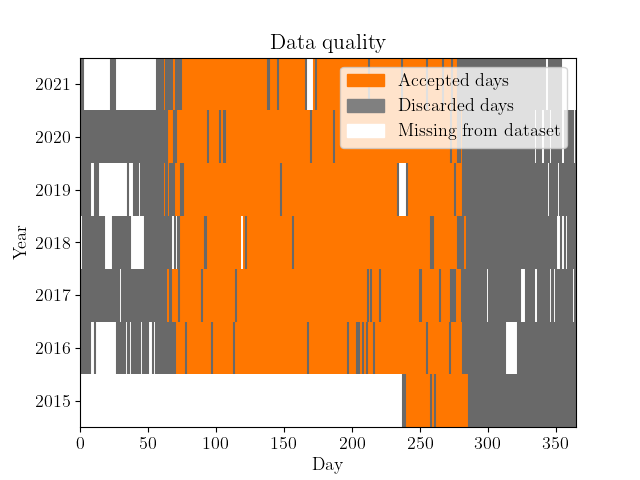
\includegraphics[width=\textwidth]{pics/helsinki_accepted_days}
         \caption{Days in Helsinki dataset which met data quality thresholds.}
         \label{fig_helsinki_accepted}
     \end{subfigure}
     \hfill
     \begin{subfigure}[b]{0.48\textwidth}
         \centering
         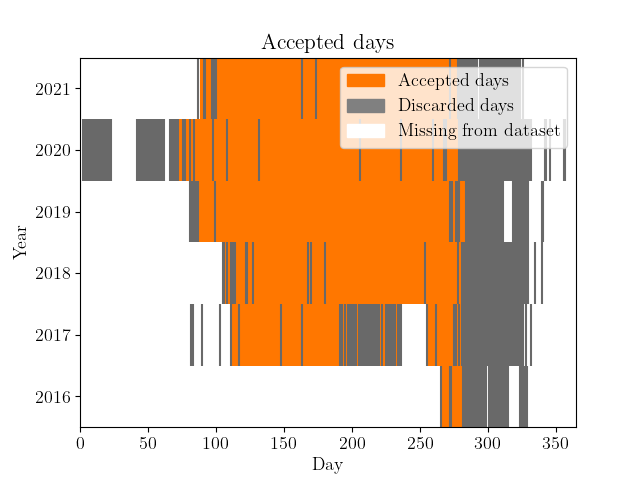
\includegraphics[width=\textwidth]{pics/kuopio_accepted_days}
         \caption{Days in Kuopio dataset which met data quality thresholds.}
         
         \label{fig_kuopio_accepted}
     \end{subfigure}
     \hfill
     \caption{Visualizations of data quality. Measurement count between 400 and 1200, first minute is 5th or later, last minute is 1435 or earlier. More than 95\% of measurements between first and last minute must be included.}
     \label{fig_accepted_days}
     
\end{figure}


After acceptable days are chosen with the classification algorithm, the next step is data repairing. Missing measurements and Nan values can be linearly interpolated, meaning that if a power measurement or a set of measurements is missing between two datapoints, the missing datapoints are estimated to describe a linear transition breaching the gap between the known datapoints. When noise level is low, linearly approximating the missing values is unlikely to result in signficant errors. After this is done, the resulting data is ready for analysis.

% One issue with the described preprocessing methods is that they do not take into account strong longitude induced shifts which may be present when installation longitudes strongly deviate from 0$^\circ$. For example, at zero degrees longitude a 12 hour day would begin at around 360 minutes and end at 1080 minutes. If the longitude is shifted by $\pm 90^\circ$, the 





%These days are then repaired by creating new days with 1440 power measurements where power at minute $i$ is the power measurement from the dataset if such measurement exists. If not, the power is defined to be 0 when outside the range of first and last non-zero measurement of the day and $Nan$ if whitin. The resulting day after these steps is defined at every minute of the day but it may still include gaps filled by $Nan$-values. These gaps 





%can be used for filling gapps in otherwise good data or for other data processing where the data is nearly usable but some modifications are needed.


%cloud free days and the topic will be better explained in the next section


%The not-a-number or $NaN$ values visible in the table \ref{table_fmi_kumpula_csv} could cause issues with some data processing algorithms. In the python programming language, many mathematical functions will always return $NaN$ if even a single $NaN$ value is present in the input. Another issue with datasets is that they include gaps, meaning that rows corresponding to some minutes are not present in the dataset. If these gaps are significant enough, their existance could causes errors and biases in processing algorithms.

%If significant amounts of measurements are missing between the first and the last measurement of the day, this could result in biases and errors with processing algorithms.


%This means that unless $NaN$ values are filtered out, a significant amount of mathematical functions will not return expected real values. Another issue with datasets is that they could include gaps, meaning that rows corresponding to some minutes are not present in the dataset. If significant amounts of measurements are missing between the first and the last measurement of the day, this could result in biases and errors with processing algorithms. %For example if a significant amount of measurements is missing, estimating the area under the plot in graphs such as \ref{fig_clearday} by simply taking the sum of the power outputs would result in underestimating the actual power output. And the more values are missing, the stronger the error would be. 

%One solution for this problem would be to design every algorithm to accept two inputs, the measured power and the measuring time but this would come at a cost to algorithm complexity. The easier option and the method used for processing the FMI datasets is the removal of all rows with $NaN$ power values and the use of linear interpolation in order to approximate the missing rows. In this case linear interpolation is applied on the minute dimension, meaning that if a gap in power measurements is detected on the minute axis, the missing minutes are filled so that the gap is filled with a linear transition breaching the gap.








\section{Clear day detection algorithm}
\label{clearskyalgo_chapter}
While the previous preprocessing steps have filtered and repaired days according to measurement counts and data gaps, these algorithms did not take other factors into account. If the interference in measurements caused by clouds or other sources is significant, the value of a day for model fitting is reduced. An example of strong interference can be seen in figure \ref{fig_cloudfree_vs_cloudy}. Detecting the presence of such interference with an algorithm would help with automating the process of model fitting as that would eliminate the need to manually select good days from datasets. The following is an explanation of how the cloud free day detection was accomplished in this thesis.




% It should be apparent that the cloudy day is not as useful for model fitting as the clear day and thus an algorithm for automating the process of detecting clear days is needed. The following steps describe the process of cloud free day detection.



%These cloud free days are visually distinct from cloudy days \ref{fig_cloudfree_vs_cloudy} and their algorithmic classification as cloud free helps in automating the parameter estimation process further. The following list is a step by step description of a such algorithm.


%\noindent \textbf{Algorithm step by step:}

\begin{enumerate}
  \item Separate the dataset into individual days.
  
  \item Create a copy of the day and apply a low pass filter to the power measurements of the copy.
  
  \item Measure the smoothness of a day by measuring how significant the changes induced by the low pass filter are.
  
  \item Discard days which fail to meet a set smoothness threshold. Remaining days are likely to be cloud free.
  
  
  
   %If the average difference from step 5 is on average higher than a given treshold value, reject the day.
\end{enumerate}



\noindent The mathematically non-trivial parts here are the threshold selection, difference measurement and low pass filtering. Low pass filtering is a term borrowed from the field of signal processing and it refers to any algorithm which removes frequencies higher than a given limit from a signal, allowing lower frequencies to pass. 

The mathematical equivalent of this process can be defined in multiple ways. In the code used for this thesis the filtering is done with the help of discrete Fourier transformations. Discrete Fourier transformation transforms a given list of numbers to a set of sine and cosine equations which approximate the given input. This trigonometric approximation can be reversed in order to return the continuous trigonometric approximation back into discrete values. As the output of a discrete fourier transformation is ordered from lowest frequency to highest, by either calculating only the first n terms or calculating all terms and zeroing out every value after term n, we can eliminate high frequencies from the continuous represenation. After this modified representation is reversed, the resulting discrete datapoints can now be said to be low pass filtered. An example of what this looks in practice is shown in figure \ref{fig_cloudfree_algo} where the 6 longest frequencies were used for approximating the discrete datapoints. 

Note that while this process is somewhat complicated, the use of fourier series is not necessary. Similar results can also be achieved by locally averaging each power value to be the average of nearest k values. Discrete Fourier transformation based methods do however have an advantage, their universality. If the 6 or 7 or n longest frequencies can be determined to be a good low pass filter, then these same frequencies should result in similar outputs no matter the temporal resolution of the power measurement data. Where as a method based on local averages would require more tuning.

The second component is not as complicated. Measuring the delta between a filtered and unfiltered set of measurements can be done by computing the discrete curve length or as was done here, measuring the absolute average deviation between filtered and unfiltered power measurement. This is shown with the following equations 2.1-2.4.


\begin{align}
Power &= [p_0, p_1, p_2, \dots , p_n] \\
Power_{filtered} &= [f_0, f_1, f_2, \dots , f_n] \\
Power_{delta} &= [|p_0 - f_0|, |p_1-f_1|, |p_2-f_2|, \dots , |p_n-f_n|] \\
delta_{avg} &= avg(Power_{delta}) \\
delta_{norm} &= delta_{avg}/ max(Power)
\end{align}


The last component is threshold selection. By choosing to reject every day for which the $delta_{norm}$ value is higher than 0.05, we can eliminate days where measurements deviate on average more than 5\% from the low pass filtered measured power values. With the Helsinki and Kuopio datasets, values as low as 0.5\% still provided some outputs. As the method is based on calculating the delta from a smooth approximation, percentual delta values are unlikely to approach zero unless the modeled data itself is faulty. Depending on the data quality, higher threshold values may need to be used. For example, if the panels are shaded by a tree or some other obstruction during a short period each day, then base level of noise in the measurements would be higher than it is for the FMI datasets.


The algorithm has weaknessess. It is designed to seek the very smoothest of days, resulting in a large amount of false negatives. In addition, other forms of interefence such as snow on panels, reflective surfaces near solar panels and clouds which do not block direct sunlight may distract the algorithm. From a human perspective the results of the algorithm may thus be unintuitive as a snowy day may be classified as cloudy even though the interference source was snow on the panels and not the cloud cover. But from the perspective of the processing algorithms, the source of noise in the data is irrelevant.

Despite these differences


%The terms used in signal processing have mathematical counterparts with some distinctions, for example we can use mathematical structures such as lists, matrices or graphs as signals. And the mathematical near equivalent of high and low frequencies could be defined with the help of delta values between neighboring numerical values in these structures. If the delta values between any two near by values is significant, then this section of the mathematical structure contains high frequency change. Similarly if delta values between any two distant values are high, this is indicative of low frequency change between these two points.






%\noindent There are two mathematically non-trivial components in the algorithm. The first is low pass filtering, a process which treats cloudy and cloud free days differently. This is a concept borrowed from the field of signal processing and the differential treatment can be used to aid in classification. The second non-trivial part is measuring the change between filtered and unfiltered measurements. If the change is minimal, the day can be classified as cloud free.

%The term low pass filtering can be used for any process which takes an input and eliminates frequencies which are higher than a chosen cut off frequency, allowing lower frequencies to pass. With the power measurements, a simple low pass filter could be a running average filter which calculates a new power value as the average of the last $n$ values. The low pass filtering used in this thesis and shown in \ref{fig_cloudfree_algo} was accomplished with discrete Fourier transformations. Discrete Fourier transformations change a list of numbers into a set of sine and cosine waves of different amplitudes, the sum of which forms a continuous representation of the discrete values. This continuous representation can be sampled in order to return the data back into discrete values and by selectively choosing only the waves with longest wavelengths, discrete Fourier transformation can be used for low pass filtering. Good results were achieved by using the 5 to 7 of the longest frequencies generated by the fast Fourier transformation algorithm. 

% n-th degree polynomial approximation of the measurements or new and filtered measurement values could be defined as the average of nearest 20 power measurements.


% The second non-trivial component is measuring the delta between filtered and unfiltered days. This is accomplished by calculating the lenghts of point to point curves in Euclidean space represented by the measurements and filtered measurements by using the equation $\Sigma_{i=1}^{n}  \sqrt[2]{1+ (powers[i]-powers[i-1])^2}$. If the curve lenghts differ by more than x percent, the day can be classified as cloudy.

%The second non-trivial component is measuring the delta between filtered and unfiltered days. This is accomplished by first computing the per minute delta $\delta[i] = |p[i] - p_{lp}[i]|$ where $p[i]$ is the measured power value at index $i$ and $p_{lp}[i]$ is the corresponding power measurement after low pass filter was applied. These delta values can then be used for calculating the average delta per measurement $\delta_{avg} = (\delta[1]+\delta[2] + \dots+ \delta[n])/n$. This normalization is important as without normalization days with lower temporal resolution or shorter day lengths would have lower delta values. The delta value $\delta_{avg}$ can be normalized further as $\delta_n=\delta_{avg}/p_{max}$. This final normalization step results in a delta which represents per measurement deviation as a fraction of max and this final value is comparable between installations of different sizes.

%Final part of cloud free day detection is choosing a threshold value. By manually testing different threshold values, the lowest values which still returns days with the Helsinki and Kuopio datasets are 0.3 and 0.5 respectively. This difference is small but it shows that there is a measurable difference between the datasets and that threshold value should be chosen based on the datasets used. Another issue with the algorithm rises from temporal resolution, if temporal resolution is 1 measurement per 15 minutes and if the reported value is an average of last measurement period, a low pass filter has already been applied. This would not make the algorithm unsuitable for its purpose, but threshold values would have to be adjusted. One method for generalizing the algorithm and avoiding the forementioned issues would be sorting the days based on their smoothness values and then choosing the $n$ smoothest days to operate on. Such modifications may be necessary or beneficial when operating with large amounts of different datasets, but as of now they have not been implemented.


%Most of the program code required for cloud free day detection is included in appendix \ref{cloudfree_code} and the complete source is available on github \cite{github_source}.

%s based on their apparent smoothness values and then operating with the 

%The second non-trivial component is measuring the delta between filtered and unfiltered days. This is accomplished by calculating the lenghts of point to point curves in euclidean space represented by the measurements and filtered measurements by using the equation $\Sigma_{i=1}^{n}  \sqrt[2]{1+ (powers[i]-powers[i-1])^2}$. If the curve lenghts differ by more than x percent


%length of a day by calculating euclidean distance over a day of measurements with the sum function: $\Sigma_{i=1}^{n}  \sqrt[2]{1+ (powers[i]-powers[i-1])^2}$



%Here the algorithm first computes the per measurement error $\delta_i$ for each measurement $p_i$ in the list of powers so that $\delta_i = |p_i - {p_i}_{lp}|$ . This results in a new list of error values is then used in orde to compute the average deviation from 



%Then the average deviation is calculated $\delta_{avg} = (\delta_1+\delta_2 + \dots+ \delta_n)/n$. Finally the delta can be normalized to 



%Here the chosen method is based on computing the length of the discrete curve in minute-power space and the equation used is the sum of point to point distances in Euclidean space. The 



%Alternative approaches such as measuring the total travel on power-axis and calculating error area between filtered and unfiltered curves could also be used. 










%The algorithm splits data into individual days of measurements and the days are evaluated separately. This means that 

%Another important form of data pre-processing is the selection of days which are suitable for model fitting. These so called cloud free or clear days can be distinguished by their smooth power measurement curves as seen in \ref{fig_cloudfree_vs_cloudy}, but the strength of cloud induced noise can be stronger or weaker as well. By making the assumption that clouds induce randomness into the power measurements, we can attempt to measure this randomness and use it as a metric for deciding whether a day is suitable for model fitting or not.

%\noindent To borrow terminology and tools from the field of signal processing, a clear difference between cloudy and cloud free days is the presense of high-frequency noise. Noise means that the alteration to the signal is unwanted and high-frequency signifies that the alteration results in a signal where measurements differ from neighboring measurements. In the case of solar PV power measurements, power $p_t$ for minute $t$ is more likely to differ from the average of the nearest 10 or 100 measurements if the day is cloudy than when the day is cloud free. This difference is visible in \ref{fig_cloudfree_algo} where a cloud free and cloudy day have both been locally averaged.

%Locally averaging or low pass filtering the values can be done in multiple ways. For example, the filtered values could be defined as the average of the nearest 50 values or a polynomial of sufficient degree could be fitted to the measurements data. Regardless of the method used, the important aspect is that the averaging function has to eliminate the apparent randomness from the signal while cloud free days should be hard to distinguish from their unfiltered counterparts. 

%Here the chosen low pass filtering method uses discrete Fourier transform. Fourier transformations are a method of representing number series and functions as sine and cosine waves. In short, the sum of a sine and a cosine wave of frequency $f$ can be used to construct a new sine wave of frequency $f$ with chosen phase. Fourier series combine this property and multiple frequencies in order to construct a frequency representation of the approximated data. As Fourier transformations start from the computation of the longest frequencies, the first $n$ outputs can be used to approximate the general shape of the data.

%This method of filtering may seem complicated as the same results could be achieved by defining new power values as $p_{t_{new}} = avg(p_{t-n}, ...,p_{t-1},  p_t,p_{t+1}, ..., p_{t+n})$ but this would require the turning of the window size parameter $n$ which is dependent on temporal resolution. The benefit of the Fourier series based method is that it is independent from temporal resolution and unlike Taylors polynomial or other localized approximation methods, discrete Fourier series approach does not favor a certain data interval.


\begin{figure}[h]
\centering
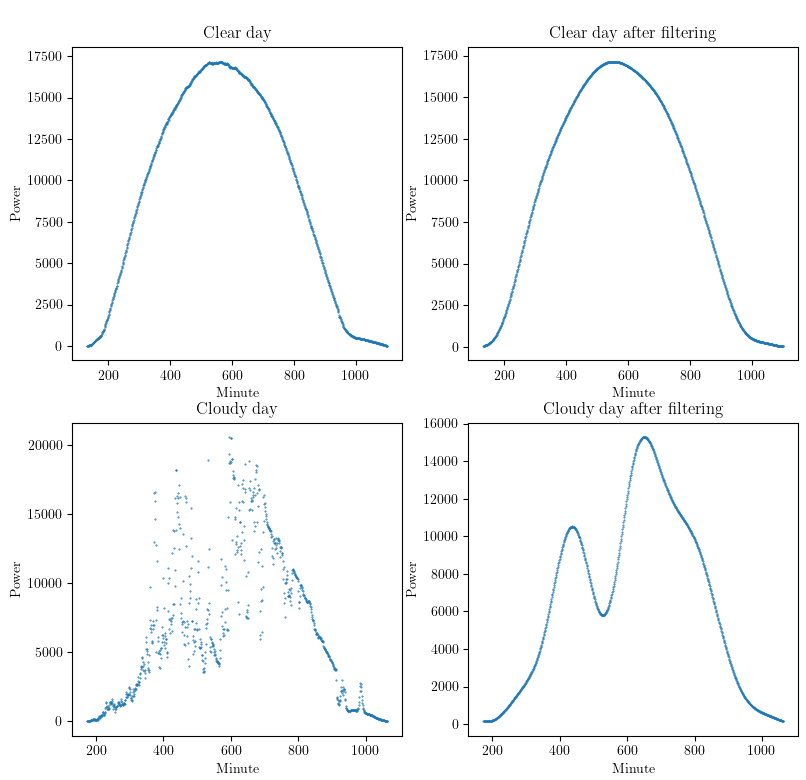
\includegraphics[width=0.8\linewidth]{pics/cloudfree_algo}
\figcaption{Cloud free day finder low pass filtering phase.}
\label{fig_cloudfree_algo}
\end{figure}



\newpage






%\noindent \textbf{Note:} that the algorithm listed above is highly dependent on measurement intervals and further tuning could be needed when operating with datasets that have different temporal resolutions. And as is, the algorithm selects days based on their proportionally low high frequency component, thus in theory this algorithm should classify zero power output days as cloud free days. Despite this fault the algorithm seems to work well for the FMI datasets.% as long as the input are selected to contain days close or between the spring and fall equinoxes. 



%The implementation of the clear sky algorithm seems to work well as indicated by \ref{fig-multidaypoavsmeasurements} but there are a few weak points in the algorithm as well. For example if a constant power day is given as the input for the algorithm, the algorithm will classify it as clear sky day even if a constant power day is more likely to be the result of faulty measuring instruments or errors in data preprocessing than a real cloud free day. In addition, the algorithm is unlikely to work well if sections are either removed from the measurements or if there is significant shading affecting the power output of the installation.

%\subsection{Difference between solar days and UTC days}
%For solar power analysis the concept of solar days is fairly useful. Solar days and sun based time measurement systems tend to rely on the angle of the sun and three 


%The timestamps used in solar PV measurements can be assumed to be in UTC +0 time. While this means that timezones or daylight saving time do not have to be accounted for, some operations may become more complicated as well since UTC days and solar days at do not always align. Note that here local solar day is defined as the 

%For example, if a one day slice is taken from a $0^\circ$ longitude installation power generation data, it is rather likely that the solar power generation would occur during an interval which centers around noon or 720 minutes. If the same slice is taken at $90^\circ$ longitude, this generation would be shifted by approximately 360 minutes. This is perfectly normal and expected behavior, but as a result, determining the first and last non-zero minutes of the day can be seen to nontrivial as per figure \ref{fig_poa0vs90}. In the $0^\circ$ plot, the first and last non-zero minutes are approximately 330 and 1100, but should the first and last minutes of the $90^\circ$ plot be defined as 0 and 750, 0 and 1420, -19 and 750 or something else entirely?


%\begin{figure}[h!]
%\centering
%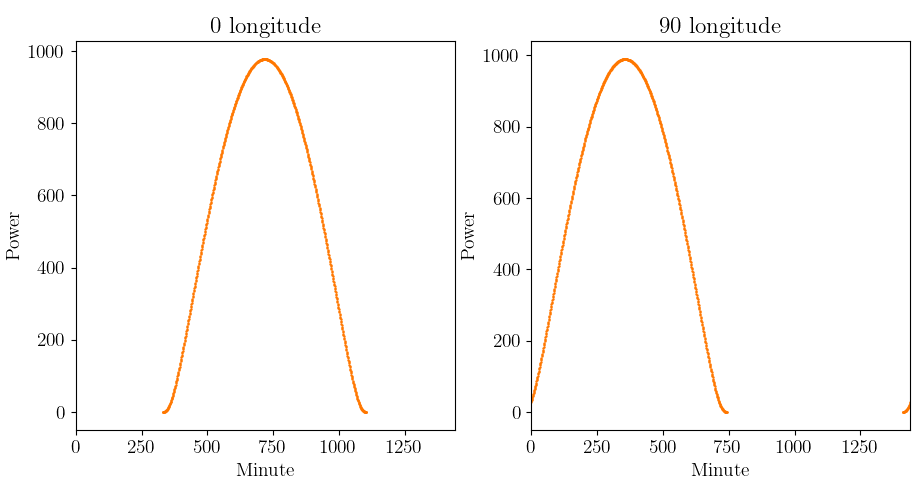
\includegraphics[width=0.9\linewidth]{pics/poa0vs90}
%\figcaption{Approximations of solar power generation at $0^\circ$ and $90^\circ$ longitude.}
%\label{fig_poa0vs90}
%\end{figure}


%\section{Third party datasets}
%Sunny portal etc here

\section{Assumptions and possible issues}
If metadata such as the geographic location or panel installation angles is missing from the datafiles, it is very likely that other critical pieces of information could be left out as well. Were additional modules were installed during operation? Could some panels be installed at different angles? What if the panels are installed in tracking mounts and thus the panel angles vary during each day? These questions are left unaswered and thus some assumptions have to be made. In this thesis we will assume that the panels are installed on fixed mounts, no changes were done during data gathering period and all panels are oriented similarly. We will also assume that there are no major obstacles casting shadows on the panels and that the panels are not self-shadowing, meaning that the panels are not casting shadows on one another.

Another source of uncertainty is data collection itself. The device responsible for measuring power output values and logging the values has to have a clock for measuring time, but this clock could have be running too slow or fast, resulting in a drifting error in the timestamps. Similarly if the system clock is running at the right speed but it is off by a minute or two, this could cause a bias in the data which would be hard to detect. There is also the question of how measurement timing is done. If the time resolution of the logging device is 15 minutes, is the power value at 12:45 taken during the 45th minute or is the power value the average of the previous 15 minutes as is often done in meteorology? Or could the power value be the average of measurements taken during the interval 12:38 to 12:52? In meoteorology, the last period average would be the standard, but standards may not always be followed.

%is the standard, but standards are not always followed and thus 

%If enough time and effort was spent on algorithm design, in theory it could be possible to detect modifications to PV systems, the presence of variable panel angle systems and clock drifts. But these topics are outside the scope of this thesis and thus the assumption will be made that the 





















